\section{The market in October 2026}\label{sec:market}

Over the P\&L window the perp fell from \BTCStart{} to \BTCEnd{} (\BTCWindow{}). The month had two phases (Figure~\ref{fig:position}):
\begin{itemize}
\item \emph{1--21 October}: a range between roughly 80{,}000 and 87{,}000, with a failed breakout early in the month and sharp intraday swings around the September CPI release on 14 October.
\item \emph{22--30 October}: a decline to below 77{,}000, with the steepest drop on the last two days.
\end{itemize}
Daily volatility was \BTCsigma{} (about 30\% annualized). The headlines the agents could read were dominated by a hot inflation print and Federal Reserve officials discussing further rate increases. The Crypto Fear \& Greed index fell from Greed (74 on 1 October) to Fear (30 at month end).

Funding on the venue stayed at its floor for \FundBase{} of the \FundPrints{} hourly prints, averaging \FundAnn{} annualized. It was negative \FundNeg{} of the time, and the average premium was \PremBp{}\,bp. A $1\times$ long therefore paid a known carry: \BHFunding{} USDC on \$100{,}000 over the month.

\section{What the desk did}\label{sec:behavior}

\paragraph{Ratings and leverage.} The portfolio manager issued \NUnderweight{} Underweight, \NOverweight{} Overweight and \NHold{} Hold ratings, and no Buy or Sell. It stated a leverage multiple on all \LevStated{} days, and every one was $1\times$ (\LevDays{} days above $1\times$). This happened although the venue contract told it to ``use leverage decisively'' when highly confident. The primary policy and its $1\times$ counterfactual therefore coincide.

Net exposure was $+0.5$ on 2--7 and 22--23 October and $-0.5$ otherwise (Figure~\ref{fig:position}), with a mean of \MeanSignedExp{}. The position changed sides five times and was otherwise left in place: \AgentTrades{} trades and a turnover of \AgentTurnover{} times equity over the month.

\paragraph{Inside the desk.} The research manager's recommendation and the PM's final rating agreed in direction on \PMeqRM{} of 30 days, and the PM toned down the research manager \PMsoftened{} time. The trader, whose schema allows only Buy, Hold or Sell, turned every Overweight into Buy and every Underweight into Sell. Read literally, those labels mean full size. The PM's text repeatedly corrected this, e.g.\ ``the trader's `Buy' label would incorrectly double the intended exposure''. The sentiment analyst rated the month Mixed on 24 of 30 days.

The pattern is that of a cautious discretionary desk. It takes half-size positions, re-decides daily, and reads mostly short-horizon technical evidence (the 10-day EMA, MACD, the perp premium), with headlines treated as unverified context.

\begin{figure}[t]\centering
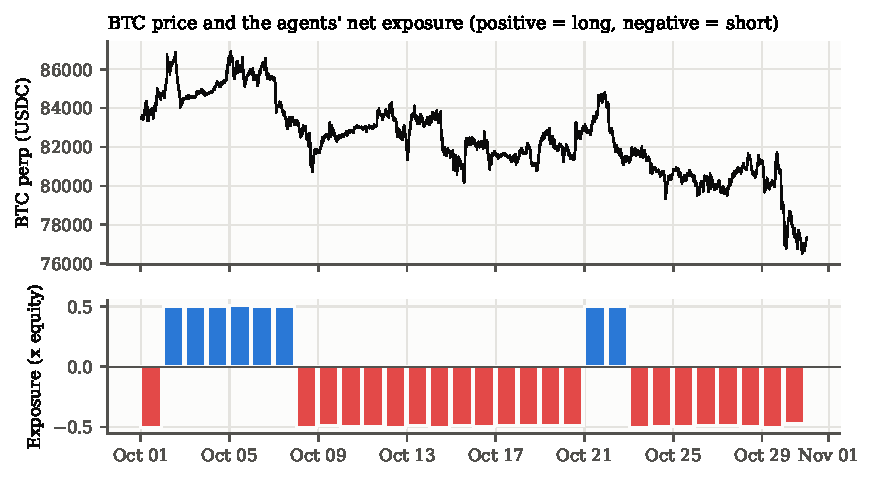
\includegraphics[width=\textwidth]{position.pdf}
\caption{BTC perp price (15-minute closes) and the desk's net exposure after each daily execution. Blue is long, red short.}\label{fig:position}
\end{figure}

\section{Performance}\label{sec:performance}

\begin{table}[t]\centering\scriptsize
\caption{Net performance, 1--31 October 2026 (\$100{,}000 start). Return is over the window; volatility, Sharpe and Sortino are annualized ($\sqrt{365}$); Max DD is measured on 15-minute marks. Turnover is total traded notional over equity. Fees include slippage; funding is in USDC (negative = received). The indented rows replay the agents' decisions under other policies; baselines decide at the same cutoffs.}\label{tab:perf}
\resizebox{\textwidth}{!}{\begin{tabular}{lrrrrrrrr}
\toprule
Strategy & Return & Vol (ann.) & Sharpe & Sortino & Max DD & Turnover & Fees & Funding \\
\midrule
TradingAgents-HL (primary, PM leverage $\le$5x) & -0.53\% & +15.3\% & -0.35 & -0.51 & -3.71\% & 4.5 & 199 & -136 \\
\quad same decisions, 1x & -0.53\% & +15.3\% & -0.35 & -0.51 & -3.71\% & 4.5 & 199 & -136 \\
\quad same decisions, long/flat 1x & -2.93\% & +9.3\% & -3.86 & -4.27 & -4.11\% & 1.8 & 80 & +149 \\
\quad same decisions, vol-target 40\% & -0.09\% & +19.7\% & 0.04 & 0.07 & -4.64\% & 6.0 & 263 & -191 \\
\quad primary + trader stop-losses & -0.76\% & +15.2\% & -0.54 & -0.80 & -3.94\% & 5.0 & 287 & -135 \\
\midrule
Buy \& hold (1x long) & -8.13\% & +30.3\% & -3.25 & -3.77 & -12.60\% & 1.0 & 45 & +708 \\
Time-series momentum (30 d) & +9.16\% & +29.9\% & 3.71 & 6.48 & -7.98\% & 3.2 & 143 & +207 \\
SMA(20) trend & -0.56\% & +30.6\% & -0.08 & -0.11 & -9.86\% & 7.1 & 313 & -259 \\
MACD histogram & +8.12\% & +30.2\% & 3.29 & 6.59 & -5.19\% & 1.3 & 57 & -718 \\
RSI(14) reversion & +0.53\% & +2.1\% & 3.14 & 34.30 & -1.26\% & 2.0 & 90 & -30 \\
Cash & +0.00\% & +0.0\% & -- & -- & +0.00\% & 0.0 & 0 & +0 \\
\bottomrule
\end{tabular}}
\end{table}

Table~\ref{tab:perf} and Figure~\ref{fig:equity} report net performance.
\begin{itemize}
\item The desk returned \AgentRet{}, with an annualized volatility of \AgentVol{} and a maximum drawdown of \AgentMDD{}.
\item Buy-and-hold returned \BHRet{}, with a drawdown of \BHMDD{}.
\item Thirty-day time-series momentum and the MACD rule were short through most of the second half and earned \TSMOMRet{} and \MACDRet{}.
\item The SMA(20) rule flipped repeatedly and finished flat.
\end{itemize}

\paragraph{Where the P\&L came from.} Figure~\ref{fig:costs} splits the desk's P\&L into price, fees, slippage and funding. Two points stand out:
\begin{itemize}
\item \emph{Trading costs were small}: \AgentFees{} USDC, including slippage, because the desk rarely traded.
\item \emph{Funding was a small gain}: the desk received \AgentFundingRecv{} USDC net. The desk was mostly short while longs paid the floor rate.
\end{itemize}

\begin{figure}[t]\centering
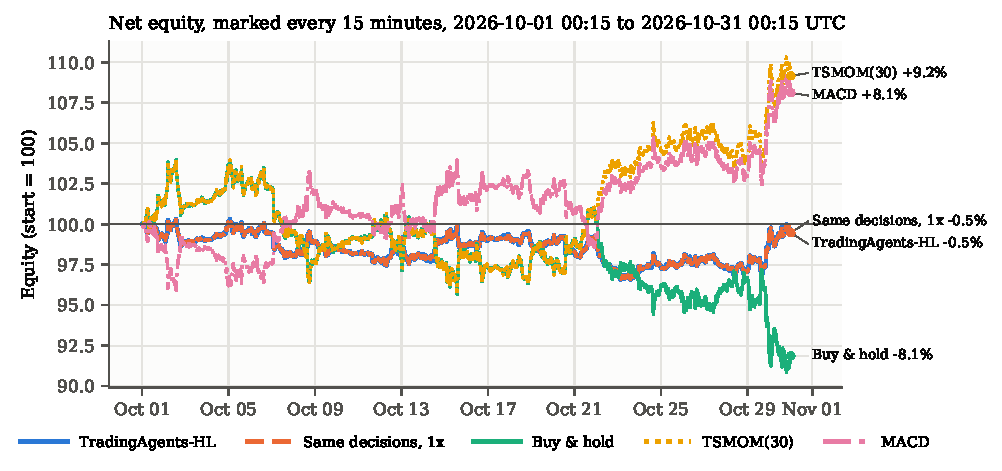
\includegraphics[width=\textwidth]{equity.pdf}
\caption{Net equity of the desk, its $1\times$ replay (identical here, as no leverage was used), buy-and-hold, and the two best baselines, marked every 15 minutes.}\label{fig:equity}
\end{figure}

\begin{figure}[t]\centering
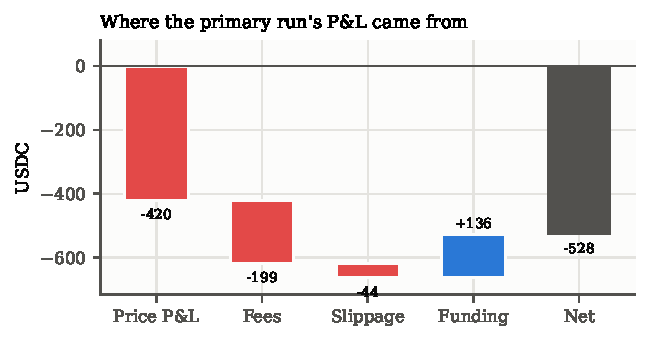
\includegraphics[width=0.62\textwidth]{costs.pdf}
\caption{The desk's P\&L, from the price move to the net result. Funding was received (positive bar) because the desk was short most of the month.}\label{fig:costs}
\end{figure}

\section{Skill or exposure?}\label{sec:skill}

Beating buy-and-hold in a falling month is easy for anyone who is short. The question is whether the desk knew \emph{when}.

\paragraph{Direction.} The desk's sign was right on \DirHits{} of \DirN{} days. The Pesaran--Timmermann statistic is \PTstat{} ($p=\PTp$), and the one-sided binomial $p$-value is \BinomP{}. Table~\ref{tab:ratings} and Figure~\ref{fig:ratings} show what followed each rating:
\begin{itemize}
\item Overweight days were followed on average by a \emph{fall} in BTC.
\item Underweight days were followed by a small fall, but up and down days were equally likely.
\end{itemize}
The rank correlation between rating and next-day return is \IC{} (permutation $p=\ICp$).

\begin{table}[t]\centering\small
\caption{What followed each PM rating: the BTC perp's return over that decision's holding period.}\label{tab:ratings}
\begin{tabular}{lrrr}
\toprule
PM rating & Days & Mean next-period BTC return & Share up \\
\midrule
Underweight & 22 & -0.15\% & 50\% \\
Hold & 1 & +1.82\% & 100\% \\
Overweight & 7 & -0.84\% & 29\% \\
\bottomrule
\end{tabular}
\end{table}

\begin{figure}[t]\centering
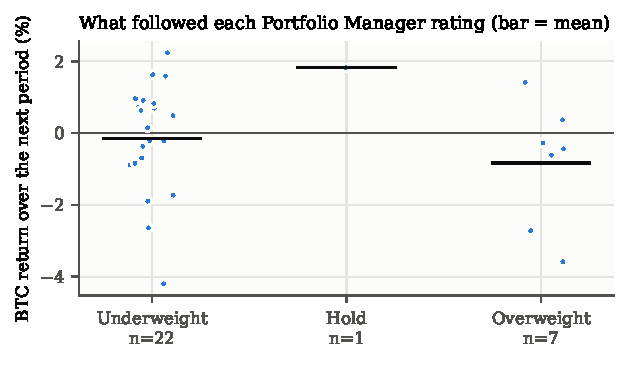
\includegraphics[width=0.62\textwidth]{ratings.pdf}
\caption{BTC return over the holding period following each rating (dots), with the mean (bar).}\label{fig:ratings}
\end{figure}

\paragraph{Exposure versus timing.} Following \citet{lo2008alphas}, the gross P\&L $\sum_t x_tR_t$ splits into two parts:
\begin{itemize}
\item a static part $T\bar x\bar R$, earned by the average exposure;
\item an active part $\sum_t(x_t-\bar x)(R_t-\bar R)$, earned by varying the exposure over time.
\end{itemize}
The desk's average exposure of \MeanSignedExp{} earned \AttrStatic{}, its timing contributed \AttrActive{}, costs \AttrCosts{} and funding \AttrFunding{}. The desk's lean was right for the month, and its timing gave that gain back.

Two features of the positions explain the timing loss:
\begin{itemize}
\item It turned long on 2 October and stayed long through the 6 October drop.
\item It turned long again on 22 October, at a local high just before the decline.
\end{itemize}
Both times the long followed a rise. The short on 7 October followed a fall.

\paragraph{Random benchmarks.} Two tests keep the desk's own propensities and destroy its timing:
\begin{itemize}
\item \emph{Permutation}: shuffling its exposures across days beats it with probability \PermGross{} gross and \PermNet{} net.
\item \emph{Random-rating Monte Carlo}: drawing each day's decision from the desk's own rating mix (\MCDraws{} draws, full engine) returns \MCmean{} on average, with a 5--95\% range of \MCqLow{} to \MCqHigh{}. The desk sits at the \MCpct{}th percentile (Figure~\ref{fig:mc}).
\end{itemize}
A random ordering of the desk's own decisions would have done better more often than not.

\begin{figure}[t]\centering
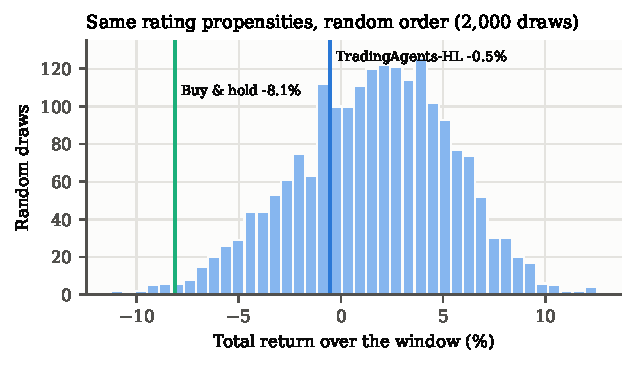
\includegraphics[width=0.62\textwidth]{montecarlo.pdf}
\caption{Net returns of \MCDraws{} random decision sequences drawn from the desk's own rating mix, against the desk and buy-and-hold.}\label{fig:mc}
\end{figure}

\paragraph{Sharpe inference.} The desk's annualized Sharpe ratio was \AgentSharpe{}, with a stationary-bootstrap 95\% interval of [\SharpeLo, \SharpeHi]. Its total return interval is [\RetLo, \RetHi]. The mean daily excess over buy-and-hold was \ExcessDaily{} [\ExcessLo, \ExcessHi]; the interval contains zero, the large realized gap notwithstanding. The other measures:
\begin{itemize}
\item probabilistic Sharpe ratio against zero: \PSR{};
\item deflated Sharpe ratio across the five policy variants: \DSR{};
\item minimum track record length: \MinTRL{}.
\end{itemize}
As the companion paper shows, with $T=\PowT$ any annualized Sharpe below about \PowMinSR{} is statistically indistinguishable from zero. This month cannot reject the hypothesis that the desk is a coin flip with a bearish tilt.

\section{Robustness}\label{sec:robust}

\paragraph{Policies.} On the same decisions (Table~\ref{tab:perf}):
\begin{itemize}
\item \emph{Long/flat} loses more: it keeps the losing longs and gives up the shorts.
\item \emph{Volatility targeting} is roughly flat.
\item \emph{Honoring the trader's stops} is slightly worse: stops closed positions on noise and paid fees twice.
\end{itemize}

\paragraph{Costs.} Table~\ref{tab:costs} varies fees and slippage. Even frictionless trading leaves the desk negative, because the desk traded so little. Costs do not explain its result, and a fee tier or staking discount would not have changed it.

\begin{table}[t]\centering\small
\caption{The primary run's decisions under alternative cost models.}\label{tab:costs}
\begin{tabular}{lrrrr}
\toprule
Cost model & Return & Sharpe & Fees & Slippage \\
\midrule
Base: tier 0 taker 4.5 bp + 1 bp slippage & -0.53\% & -0.35 & 199 & 44 \\
Taker, no slippage & -0.48\% & -0.31 & 199 & 0 \\
Slippage 2 bp & -0.57\% & -0.38 & 199 & 89 \\
Slippage 5 bp & -0.71\% & -0.49 & 199 & 221 \\
Fee tier 3 (3.0 bp taker) & -0.46\% & -0.29 & 133 & 44 \\
Tier 6 + Diamond staking (1.44 bp) & -0.39\% & -0.24 & 64 & 44 \\
All fills as maker (1.5 bp) & -0.35\% & -0.20 & 66 & 0 \\
Frictionless (no fee, no slippage) & -0.28\% & -0.15 & 0 & 0 \\
\bottomrule
\end{tabular}
\end{table}

\paragraph{Leverage.} Table~\ref{tab:fixedlev} replays the same decisions with a fixed leverage multiple applied to every directional rating. This is a risk sensitivity, not a strategy: choosing the multiple after seeing the outcome would be look-ahead by the researcher.
\begin{itemize}
\item Leverage scales the loss and the fees without changing the sign.
\item At $20\times$ (positions of about $10\times$ equity, because the ratings were half-size) the account loses about 40\%, with a drawdown near two thirds.
\item At the venue's $40\times$, the account is liquidated on 21 October.
\end{itemize}
The desk's refusal to use leverage was, in hindsight, its most valuable decision.

\begin{table}[t]\centering\small
\caption{The same decisions with a fixed leverage multiple on every directional rating, with liquidation enforced on 15-minute bars at the venue's maintenance margin.}\label{tab:fixedlev}
\begin{tabular}{rrrrrrl}
\toprule
Multiple $L$ & Max position & Return & Sharpe & Max DD & Fees & Liquidated \\
\midrule
1x & 0.5x & -0.53\% & -0.35 & -3.71\% & 199 & no \\
2x & 1.0x & -1.09\% & -0.29 & -7.31\% & 397 & no \\
5x & 2.5x & -4.71\% & -0.40 & -18.49\% & 1,019 & no \\
10x & 5.0x & -13.80\% & -0.44 & -36.03\% & 2,022 & no \\
20x & 10.1x & -39.57\% & -0.50 & -64.91\% & 3,686 & no \\
40x & 20.7x & -95.52\% & -3.11 & -95.63\% & 5,113 & 2026-10-21 \\
\bottomrule
\end{tabular}
\end{table}

\section{Leakage audit}\label{sec:leakage}

\paragraph{Data path.} Four checks cover the data the agents read.
\begin{itemize}
\item \emph{Canary test.} It feeds every venue tool two synthetic histories that are identical before the cutoff and absurd after it, and passes: no tool output changes.
\item \emph{News lag.} The newest headline any decision could read was a median of \NewsAgeMed{} hours old at its cutoff (maximum \NewsAgeMax{}). The other items were held back by the known-at rule, which affects the \NewsDateOnly{} of headlines stamped by date only.
\item \emph{Memory.} Every lesson in the memory log was visible only from its resolution date, two decisions after the decision it concerns. The run log records each settlement before the decision that first reads it.
\item \emph{Replay.} Replaying the ledger reproduces the recorded equity exactly, so no input changed between the run and this analysis.
\end{itemize}

\paragraph{Clock.} Asked for today's date with no date given, \texttt{gpt-6-sol} answered UNKNOWN and \texttt{gpt-6-luna} invented a date in 2025. Neither was told the real date by the provider.

\paragraph{Memorization.} We asked each model for Bitcoin's daily close on every day of the window, and on the 15th of each month from August 2025 to April 2026, as controls. A first probe of ten dates allowed the answer UNKNOWN, and both models declined every date, including the controls. Forced to give a number, they produced the results in Table~\ref{tab:leak}.

\begin{table}[h]\centering\small
\caption{Forced price estimates. Errors are medians of $|\hat P/P-1|$ over 9 controls and 30 window days. ``Guessed'' and ``realized'' changes run from 1 to 30 October. ``Corr.'' is the correlation between guessed and realized closes over the window, with a Fisher-$z$ $p$-value.}\label{tab:leak}
\begin{tabular}{lrrrrr}
\toprule
Model & Control error & Window error & Guessed change & Realized change & Corr. ($p$) \\
\midrule
\texttt{gpt-6-luna} & 6.4\% & 22.8\% & -5.0\% & -8.8\% & +0.31 (0.10) \\
\texttt{gpt-6-sol} & 0.1\% & 10.0\% & +11.8\% & -8.8\% & -0.24 (0.19) \\
\bottomrule
\end{tabular}
\end{table}

The larger model has memorized prices: its control error is 0.1\%. It recalls month-end closes from August 2025 to January 2026 almost exactly. From February 2026 its error jumps to 20--30\%, so its effective knowledge of prices ends about three months before its reported cutoff.

On October 2026 its guesses are a flat \$75--95k with no relation to the realized path: a 10\% median error and a correlation of $-0.24$. Its guesses rise 12\% over the month while the price fell 9\%.

The smaller model knows less even before its cutoff. In October it guesses between \$75k and \$125k with a 23\% median error. Its weak positive correlation ($+0.31$, $p=0.10$) is not significant, before any correction for testing two models.

A model that knew October would show the precision it shows on its controls. Neither does.

\section{Sampling noise}\label{sec:consistency}

Each decision is one sample from a stochastic system, so a different sample could have produced a different month. We re-ran every sixth decision (\ConsN{} dates) on identical inputs:
\begin{itemize}
\item the same cutoff and cached data;
\item the book the original run saw;
\item the memory log as it stood then, with the decision itself removed.
\end{itemize}
Only the models' sampling differed.

\begin{table}[h]\centering\small
\caption{Original and re-run decisions on identical inputs.}\label{tab:cons}
\begin{tabular}{lllll}
\toprule
Date & Original & Lev. & Re-run & Lev. \\
\midrule
2026-10-05 & Overweight & 1.0 & Overweight & 1.0 \\
2026-10-11 & Underweight & 1.0 & Underweight & 1.0 \\
2026-10-17 & Underweight & 1.0 & Underweight & 1.0 \\
2026-10-23 & Underweight & 1.0 & Underweight & 1.0 \\
2026-10-29 & Underweight & 1.0 & Underweight & 1.0 \\
\bottomrule
\end{tabular}
\end{table}

All \ConsSame{} re-runs reproduced the original rating and leverage (Table~\ref{tab:cons}). The desk is therefore not a coin flip from one sample to the next.

Two caveats limit this:
\begin{itemize}
\item Four of the five dates fall in the long short regime, and the book the desk reads shows the position already held, which may anchor it.
\item With five pairs, 5/5 agreement only establishes, at 95\% confidence, that the desk gives the same rating at least 55\% of the time ($0.05^{1/5}\approx0.55$).
\end{itemize}
Within these limits, the month's result reflects the desk's policy more than its sampling noise. It also means the desk's poor timing would likely recur on a re-run.


\section{Three decisions}\label{sec:cases}

\paragraph{6 October (Overweight, BTC $-2.72\%$).} With the book already at $+0.5\times$, the PM kept it:
\begin{quote}\small
``The modest-long case wins on direction: BTC-USD remains above its \$84,831 10-day EMA, \$83,845 Bollinger middle and rising \$79,910 50-day average, with a +6.52\% 30-day return and RSI of 63.48. But two softer closes, a negative MACD histogram, volume at 0.70$\times$ average and a modest $-1.85$\,bp perp premium leave an \$88,000 breakout unconfirmed; they cap conviction rather than establish a short thesis.''
\end{quote}
It also cited the \$2{,}161 ATR as a reason not to lever. BTC fell 2.7\% over the next 24 hours, the desk's worst day.

\paragraph{7 October (Underweight, BTC $-1.73\%$).} After that drop the desk flipped, with an explicit cost estimate:
\begin{quote}\small
``From the current approximately +50\% long, sell approximately 1$\times$ equity of BTC-USD notional (about 98,100 USDC at the quoted mark), including closing the long; estimated execution cost is about 54 USDC at 5.5\,bp.''
\end{quote}
The flip followed the move rather than anticipating it. It was nevertheless right for the next day.

\paragraph{28 October (Underweight, BTC $-4.20\%$).} The desk kept its short, which needed no trade, through the month's largest drop. It listed what would make it wrong (``a sustained reclaim of the \$81,556 VWMA and \$81,919 50-day SMA'') and why it was not shorting harder (one- and three-day gains, price above the 200-day average). This was its best day, at $+2.1\%$.

These excerpts show the desk's strengths: numbers grounded in tools, explicit invalidation levels, awareness of costs and of the venue contract. They also show its weakness: its evidence is mostly the recent path of the price, and it reacts to moves rather than anticipating them.

\section{Discussion and limitations}\label{sec:discussion}

\paragraph{What this month shows.} An LLM desk given an honest information set and honest costs behaved like a prudent discretionary trader. It sized small, refused leverage, explained itself, and preserved capital in a falling market. It showed no ability to time daily moves: its gross result is a correct average stance, a negative timing component, and statistics consistent with chance. Simple trend rules did better this month. One month, however, cannot rank strategies; a trending month is exactly when trend rules shine.

\paragraph{Limitations.}
\begin{itemize}
\item \emph{Sample.} Thirty observations give very low power (\S\ref{sec:skill}).
\item \emph{One path.} Each day is one sample of a stochastic system; Section~\ref{sec:consistency} measures how often it changes its mind.
\item \emph{Counterfactual policies.} These replay decisions that were conditioned on the primary book.
\item \emph{Slippage} is modeled, not observed.
\item \emph{News} are headlines only, ranked by a search engine at fetch time, and lag by up to 17 hours.
\item \emph{FRED macro series} were not configured (no API key). The news analyst was told the data was unavailable, and macro events still reached it through headlines.
\item \emph{Prediction-market data} is live-only and was withheld.
\item \emph{Memory} started empty.
\item \emph{One model pair}: the results concern one pair of models through one provider.
\end{itemize}

\paragraph{Future work.} The natural next steps are:
\begin{itemize}
\item a longer walk-forward window, which is the only way to gain power;
\item repeated sampling of each day, to separate the desk's policy from its noise;
\item hourly decisions with maker execution;
\item an ablation of each analyst, to find which inputs, if any, carry information.
\end{itemize}

\section{Conclusion}
Over October 2026 the TradingAgents desk on Hyperliquid returned \AgentRet{} while Bitcoin fell \BTCWindow{}. It kept its drawdown to \AgentMDD{} and never touched leverage. Its outperformance over buy-and-hold came from a bearish lean, not from timing. Every test of timing is consistent with chance, and the leverage the venue offers would have wiped it out. The value of the exercise lies less in the number than in the procedure: a month of LLM decisions, priced honestly and audited for leakage, whose result is reported with the uncertainty it carries.
